% Compilar com: latexmk -pdf Apresentacao_Atividade_2_Beamer.tex
\documentclass[aspectratio=169,11pt]{beamer}

\usepackage[utf8]{inputenc}
\usepackage[T1]{fontenc}
\IfFileExists{brazil.ldf}{\usepackage[brazil]{babel}}{\usepackage[english]{babel}\frenchspacing}
\usepackage{mathpazo}
\IfFileExists{eulervm.sty}{\usepackage{eulervm}}{}
\usepackage{booktabs}
\usepackage{tabularx}
\usepackage{array}
\usepackage{tikz}
\usetikzlibrary{positioning}
\usepackage{listings}
\usepackage{xcolor}

\usetheme{Dresden}
\usefonttheme{serif}
\usecolortheme{rose}

\setbeamertemplate{navigation symbols}{}
\setbeamertemplate{caption}[numbered]
\setbeamerfont{title}{size=\LARGE,series=\bfseries}
\setbeamerfont{frametitle}{series=\bfseries}
\setbeamerfont{footnote}{size=\tiny}

\definecolor{codigoFundo}{RGB}{247,247,249}
\definecolor{roseaccent}{RGB}{176,74,110}
\lstset{
  basicstyle=\ttfamily\scriptsize,
  backgroundcolor=\color{codigoFundo},
  frame=single,
  rulecolor=\color{gray!35},
  columns=fullflexible,
  keepspaces=true,
  showstringspaces=false,
  breaklines=true
}

\newcolumntype{Y}{>{\raggedright\arraybackslash}X}

\title{Atividade 2: Analisador Léxico}
\subtitle{Implementação para a linguagem Mini\_Pascal}
\author{João Paulo Sandes Brito}
\institute[UESB -- Compiladores]{Universidade Estadual do Sudoeste da Bahia\\Disciplina de Compiladores}
\date{2026.2}

\begin{document}

\begin{frame}
  \titlepage
\end{frame}

\begin{frame}{Roteiro}
  \tableofcontents
\end{frame}

\section{Objetivo}

\begin{frame}[fragile]{Entrada, análise e saída}
  \begin{columns}[T,onlytextwidth]
    \column{0.56\textwidth}
      \begin{block}{Objetivo}
        Reconhecer os lexemas de um programa Mini\_Pascal e atribuir a cada um sua classe léxica.
      \end{block}

      \begin{itemize}
        \item Implementação em Java 17;
        \item transições determinísticas;
        \item interface gráfica com Swing;
        \item modo de linha de comando.
      \end{itemize}

    \column{0.40\textwidth}
      \begin{alertblock}{Saída}
        Um par \textbf{lexema--token} por linha.
      \end{alertblock}

      \begin{lstlisting}
program - Palavra reservada
media   - Identificador
:=      - Atribuicao
24.5    - Numero real
      \end{lstlisting}
  \end{columns}
\end{frame}

\section{Reconhecimento}

\begin{frame}{Classes léxicas}
  \small
  \begin{tabularx}{\textwidth}{p{3.1cm}Y Y}
    \toprule
    \textbf{Classe} & \textbf{Exemplos} & \textbf{Resultado} \\
    \midrule
    Palavra reservada & \texttt{program}, \texttt{begin} & Palavra reservada \\
    Identificador & \texttt{x}, \texttt{media\_geral} & Identificador \\
    Número & \texttt{13}, \texttt{24.40e-04} & Inteiro ou real \\
    Constante & \texttt{'A'}, \texttt{"texto"} & Caractere ou string \\
    Operador & \texttt{+}, \texttt{>=}, \texttt{and} & Aritmético, relacional ou lógico \\
    Símbolo & \texttt{( ) , ; :}, \texttt{:=}, \texttt{.} & Especial, atribuição ou fim \\
    \bottomrule
  \end{tabularx}

  \vspace{0.5em}
  \footnotesize Espaços, tabulações, quebras de linha e comentários não produzem tokens.
\end{frame}

\begin{frame}{Estrutura e fluxo do analisador}
  \begin{columns}[T,onlytextwidth]
    \column{0.44\textwidth}
      \begin{block}{Componentes}
        \begin{itemize}
          \item \texttt{Lexer}: reconhecimento;
          \item \texttt{Token}: resultado;
          \item \texttt{AnalysisFileService}: arquivos;
          \item \texttt{MainFrame}: interface;
          \item \texttt{Main}: inicialização.
        \end{itemize}
      \end{block}

    \column{0.52\textwidth}
      \centering
      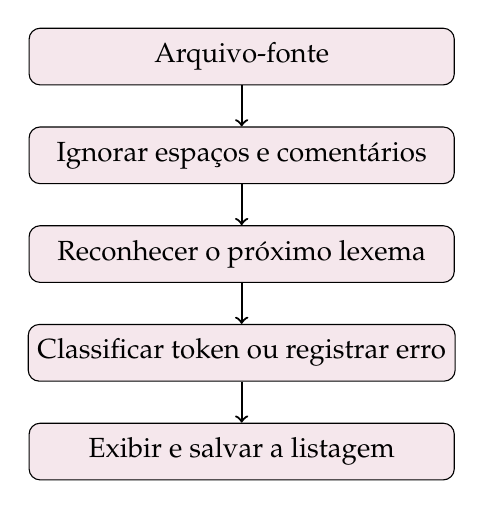
\begin{tikzpicture}[
        node distance=0.52cm,
        caixa/.style={draw,rounded corners,fill=roseaccent!13,minimum width=5.4cm,minimum height=0.72cm,align=center},
        seta/.style={->,thick}
      ]
        \node[caixa] (entrada) {Arquivo-fonte};
        \node[caixa,below=of entrada] (ignorar) {Ignorar espaços e comentários};
        \node[caixa,below=of ignorar] (reconhecer) {Reconhecer o próximo lexema};
        \node[caixa,below=of reconhecer] (classificar) {Classificar token ou registrar erro};
        \node[caixa,below=of classificar] (saida) {Exibir e salvar a listagem};
        \draw[seta] (entrada) -- (ignorar);
        \draw[seta] (ignorar) -- (reconhecer);
        \draw[seta] (reconhecer) -- (classificar);
        \draw[seta] (classificar) -- (saida);
      \end{tikzpicture}
  \end{columns}
\end{frame}

\section{Erros}

\begin{frame}{Tratamento de erros léxicos}
  \begin{columns}[T,onlytextwidth]
    \column{0.48\textwidth}
      \begin{block}{Informações registradas}
        \begin{itemize}
          \item lexema problemático;
          \item linha e coluna;
          \item descrição do erro.
        \end{itemize}
      \end{block}

      \begin{alertblock}{Recuperação}
        A unidade inválida é consumida e a análise continua no próximo ponto seguro.
      \end{alertblock}

    \column{0.48\textwidth}
      \begin{block}{Casos detectados}
        \begin{itemize}
          \item símbolo desconhecido;
          \item expoente incompleto;
          \item número unido a identificador;
          \item comentário ou string sem fechamento;
          \item constante caractere inválida.
        \end{itemize}
      \end{block}
  \end{columns}
\end{frame}

\section{Execução}

\begin{frame}[fragile]{Interface e execução no Windows}
  \begin{columns}[T,onlytextwidth]
    \column{0.51\textwidth}
      \begin{block}{Interface gráfica}
        \begin{enumerate}
          \item Abrir o arquivo-fonte;
          \item executar a análise;
          \item conferir lexema, token e posição;
          \item salvar a listagem.
        \end{enumerate}
      \end{block}

      \begin{itemize}
        \item Botões: \textbf{Abrir arquivo}, \textbf{Analisar}, \textbf{Salvar tokens} e \textbf{Limpar}.
      \end{itemize}

    \column{0.45\textwidth}
      \begin{block}{Execução direta}
        \texttt{executar.bat}
      \end{block}

      \begin{block}{Linha de comando}
        \begin{lstlisting}
java -jar dist\MiniPascal-Lexico.jar entrada.txt saida.txt
        \end{lstlisting}
      \end{block}

      \footnotesize Requisito: Java 17 ou superior. Nenhuma IDE é necessária.
  \end{columns}
\end{frame}

\section{Verificação}

\begin{frame}{Testes executados}
  \begin{columns}[T,onlytextwidth]
    \column{0.58\textwidth}
      \small
      \begin{tabular}{lrr}
        \toprule
        \textbf{Caso} & \textbf{Tokens} & \textbf{Erros} \\
        \midrule
        Programa básico & 50 & 0 \\
        Números e constantes & 48 & 0 \\
        Operadores & 74 & 0 \\
        Comentários & 15 & 0 \\
        Erros léxicos & 30 & 5 \\
        Caixa e Unicode & 32 & 0 \\
        \midrule
        \textbf{Total} & \textbf{249} & \textbf{5} \\
        \bottomrule
      \end{tabular}

    \column{0.38\textwidth}
      \begin{block}{Resultado}
        \begin{itemize}
          \item 6 arquivos de entrada;
          \item 20 verificações automatizadas;
          \item 6 saídas iguais às referências;
          \item erros do quinto caso inseridos intencionalmente.
        \end{itemize}
      \end{block}
  \end{columns}
\end{frame}

\begin{frame}{Conclusão}
  \begin{itemize}
    \item As classes léxicas definidas para Mini\_Pascal foram reconhecidas.
    \item Os erros registram posição e mensagem sem interromper toda a análise.
    \item A interface e o JAR permitem executar o programa diretamente no Windows.
    \item A separação entre léxico, arquivos e interface facilita as próximas etapas do compilador.
  \end{itemize}

  \vfill
  \begin{center}
    \Large\textbf{Obrigado.}
  \end{center}
\end{frame}

\end{document}
